\documentclass[letterpaper, 10 pt, conference]{ieeeconf}

\usepackage{amsfonts,amsmath,amssymb}
\usepackage{bm}
\usepackage{float}
\usepackage{graphicx}
\usepackage{color}
%\usepackage[dvipdfmx]{hyperref}
\usepackage{algorithm}
\usepackage{algorithmic}
%\usepackage{txfonts}
%\usepackage{ascmac, here}
\usepackage{listings}
\usepackage{color}
%\usepackage{url}
\usepackage{comment}

\allowdisplaybreaks[1]

\newtheorem{theorem}{Theorem}
\newtheorem{corollary}{Corollary}
\newtheorem{lemma}{Lemma}
\newtheorem{prop}{Proposition}
\newtheorem{definition}{Definition}

%\theoremstyle{definition}
%\newtheorem{definition}{Definition}[section]

%\theoremstyle{remark}
%\newtheorem*{remark}{Remark}

\newcommand{\mysps}{\ensuremath{[\![s^{\otimes}]\!]}_s}
\newcommand{\myspq}{\ensuremath{[\![s^{\otimes}]\!]}_q}
\newcommand{\myspds}{\ensuremath{[\![s^{\otimes \prime}]\!]}_s}
\newcommand{\myspdq}{\ensuremath{[\![s^{\otimes \prime}]\!]}_q}
\newcommand{\argmax}{\mathop{\rm arg~max}\limits}
\newcommand{\argmin}{\mathop{\rm arg~min}\limits}

\begin{document}

\section{System Model}

\begin{definition}
We represent a probabilistic discrete event systems (DES) as a labeled Markov decision process (MDP). A DES is a tuple $M$ = $(S, E, \mathcal{E}, P_T, s_{init}, AP, L)$, where S is a finite set of states; $E$ is a finite set of events; $\mathcal{E} : S \rightarrow E$ is a mapping that maps each state to the set of feasible events at the state; $P_T:S \times S \times E \rightarrow [0,1]$ is a transition probability such that $\sum_{s' \in S} P_T(s'|s,e) = 1$ for any state $s \in S$ and any event $e \in \mathcal{E}(s) $ and such that $P_T(s'|s,e) = 0$ for any $e \notin \mathcal{E}(s)$; $s_{init} \in S$ is the initial state; $AP$ is a finite set of atomic propositions; and $L : S \times E \times S \rightarrow 2^{AP}$ is a labeling function that assigns a set of atomic propositions to each transition $(s, e, s') \in S \times E \times S$. We assume that $E$ can be partitioned into the set of controllable events $E_c$ and the set of uncontrollable events $E_{uc}$ such that $E_c \cup E_{uc} = E$ and $E_c \cap E_{uc} = \emptyset$. Note that each event $e$ occurs probabilistically depending on only the current state and the subset of feasible events at the state. We define a reward function $\mathcal{R} : S \times 2^E \times E \times S \rightarrow \mathbb{R}$.

In the DES $M$, an infinite path starting from a state $s_0 \in S$ is defined as a sequence $\rho\ =\ s_0e_0s_1 \ldots\ \in S (E S)^{\omega}$ such that $P_T(s_{i+1}|s_i, e_i) > 0$ for any $ i \in \mathbb{N}_0$, where $\mathbb{N}_0$ is the set of natural numbers including zero A finite path is a finite sequence in $S (E S)^*$. In addition, we sometimes represent $\rho$ as $\rho_{init}$ to emphasize that $\rho$ starts from $s_0 = s_{init}$.
For a path $\rho\ =\ s_0e_0s_1 \ldots$, we define the corresponding labeled path $L(\rho)\ =\ L(s_0,e_0,s_1)L(s_1,e_1,s_2) \ldots \in (2^{AP})^{\omega}$.
% We define the set of finite labeled paths as $\mathcal{L}(M) = \{ L(\rho) \in (2^{AP})^{\omega} ; \rho = s_0e_0s_1 \ldots \in S(ES)^{\ast},\ P(s_{i+1}|s_i, e_i) > 0,\ i \in \mathbb{N}_0  \}.
 $InfPath^{M}\ ( \text{resp., }FinPath^{M})$ is defined as the set of infinite (resp., finite) paths starting from $s_0=s_{init}$ in the DES $M$. For each finite path $\rho$, $last(\rho)$ denotes its last state.
\end{definition}

\begin{definition}
For the DES $M$,  we define a supervisor $SV : FinPath^{M} \rightarrow 2^E$ is a mapping that maps each finite path to a set of allowed events at the finite path and we call the set the control pattern. In the following, the supervisor we consider is {\it state-based}, namely for any $\rho \in FinPath^{M}$, $SV(\rho) = SV(last(\rho))$.
\end{definition}

\begin{definition}
  A sink state in state set $X$ of an augmented tLDBA $\bar{B}_{\varphi} = (\bar{X}, \bar{x}_{init},\bar{\Sigma},\bar{\delta},\bar{\mathcal{F}})$ is defined as a state such that there exist no accepting transition of $\bar{B}_{\varphi}$ that is accessible from the state. We denote the set of sink states as $Sink Set$.
\end{definition}

\begin{definition}
  Given an augmented tLDBA $\bar{B}_{\varphi} = (\bar{X}, \bar{x}_{init},\bar{\Sigma},\bar{\delta},\bar{\mathcal{F}})$ and a DES $M$, a tuple $M \otimes \bar{B}_{\varphi} = M^{\otimes} = (S^{\otimes}, E^{\otimes}, {\mathcal E}^{\otimes}, s_{init}^{\otimes}, P^{\otimes}_T, \delta^{\otimes}, {\mathcal F}^{\otimes})$ is a product DES, where
  $S^{\otimes} = S \times \bar{X}$ is the finite set of states and we represent $s$ and $\bar{x}$ corresponding with $s^{\otimes} = (s,\bar{x}) \in S^{\otimes}$ as $\mysps$ and $\myspq$, respectively, $E^{\otimes}=E$ is the finite set of events, ${\mathcal E}^{\otimes} : S^{\otimes} \rightarrow 2^{E^{\otimes}}$ is the mapping defined as ${\mathcal E}^{\otimes}((s,\bar{x})) = {\mathcal E}(s)$, $s_{init}^{\otimes} = (s_{init},\bar{x}_{init})$ is the initial states, $P^{\otimes}_T : S^{\otimes} \times S^{\otimes} \times E^{\otimes} \rightarrow [0,1]$ is the transition probability defined as
  \begin{align}
    P^{\otimes}_T(s^{\otimes \prime} | s^{\otimes}, e) =
    \left\{
    \begin{aligned}
      &P_T(s^{\prime} | s, e) &   &\text{if}\  (\bar{x}, L((s,e,s^{\prime})), \bar{x}^{\prime}) \in \bar{\delta},\\
      &0 &   &\text{otherwise} ,
    \end{aligned}
    \right. \nonumber
  \end{align}
  $\delta^{\otimes} = \{ (s^{\otimes}, e, s^{\otimes \prime}) \in S^{\otimes} \times E^{\otimes} \times S^{\otimes} ; P^{\otimes}_T(s^{\otimes \prime} | s^{\otimes}, e) > 0 \}$ is the set of transitions, and ${\mathcal F}^{\otimes} = \{ \bar{F}^{\otimes}_1, \ldots ,\bar{F}^{\otimes}_n \}$ is the acceptance condition, where $\bar{F}^{\otimes}_i = \{ ((s,\bar{x}), e, (s^{\prime}, \bar{x}^{\prime})) \in \delta^{\otimes}\ ;\ (\bar{x}, L(s,e,s^{\prime}), \bar{x}^{\prime}) \in \bar{F}_i \}$ for each $ i \in \{ 1, \ldots ,n \}$.
\end{definition}

\section{Objective function for Control patterns}
From the view point of reinforcement learning, the DES can be interpreted as the environment controlled by the supervisor and the supervisor can be interpreted as the agent. We introduce that the three following assumptions.

\begin{enumerate}
  \item state transitions in the DES occur after a probabilistic occurrence of an event. Therefore, for any $(s^{\prime}, s, \pi) \in S \times S \times 2^E$, we assume that the following equation.
  \begin{align}
    P(s'|s,\pi) = \sum_{e \in \pi}P_1(e|s,\pi) P_T(s^{\prime}|s,e),
  \end{align}
  where $P_1 : E \times S \times 2^E$ is the probability that an event occurs after a control pattern $\pi \in \mathcal{E}(s)$ is selected by the supervisor at the state $s \in S$ and $P : S \times S \times 2^E$ is interpreted as the probability that a state transition occurs under that the control pattern is given by the supervisor at the current state.

  \item The probability of occurrence of each event does not depend on the control pattern. We introduce a parameter $\eta : S \times E \rightarrow \mathbb{R}_{>0}$ that represents the frequency of occurrence of the event $e \in E$ at the state $s \in S$, where $\mathbb{R}_{>0}$ is the set of positive real values. Then, for any $(e,s,\pi) \in E \times S \times 2^E$, we assume that the following equation.
  \begin{align}
    P_1(e|s,\pi) = \frac{\eta(s,e)}{\sum_{e^{\prime} \in \pi} \eta(s,e^{\prime})}.
  \end{align}

  \item The reward $\mathcal{R}$ can be decomposed into $\mathcal{R}_1$ and $\mathcal{R}_2$. The first reward $\mathcal{R}_1 : S \times 2^E \rightarrow \mathbb{R}$ is the reward that is determined by the control pattern selected by the supervisor, which depends on only the control pattern and current state. The second reward $\mathcal{R}_2 : S \times E \times S \rightarrow \mathbb{R}$ is the reward that is determined by the occurrence of an event and the corresponding state transition. For any $(s,\pi,e,s^{\prime}) \in S \times 2^E \times E \times S$, we then have
  \begin{align}
    \mathcal{R}(s,\pi,e,s^{\prime}) = \mathcal{R}_1(s,\pi) + \mathcal{R}_2(s,e,s^{\prime}).
  \end{align}
\end{enumerate}
Under the assumptions, we have the following {\it Bellman optimality equation}.

\begin{align}
  Q^{\ast}(s,\pi) = & \sum_{s^{\prime} \in S} \left[ \sum_{e \in \pi} P_1(e|s,\pi) P_2(s^{\prime}|s,e) \right. \nonumber \\
  & \left. \left \{ \mathcal{R}(s,\pi,e,s^{\prime}) + \gamma \max_{\pi^{\prime} \in 2^{\mathcal{E}(s^{\prime})}} Q^{\ast}(s^{\prime},\pi^{\prime}) \right \} \right] \nonumber \\
  = & \sum_{s^{\prime} \in S} \left[ \sum_{e \in \pi} P_1(e|s,\pi) P_2(s^{\prime}|s,e) \right. \nonumber \\
  & \left. \left \{ \mathcal{R}_1(s,\pi) + \mathcal{R}_2(s,e,s^{\prime}) + \gamma \max_{\pi^{\prime} \in 2^{\mathcal{E}(s^{\prime})}} Q^{\ast}(s^{\prime},\pi^{\prime}) \right \} \right] \nonumber \\
  = & \mathcal{R}_1(s,\pi) + \sum_{e \in \pi}P_1(e|s,\pi) \left[ \sum_{s^{\prime \in S}} P_2(s^{\prime}|s,e)) \right. \nonumber \\
  & \left. \left \{ \mathcal{R}_2(s^{\prime}|s,e) + \gamma \max_{\pi^{\prime} \in 2^{\mathcal{E}(s^{\prime})}} Q^{\ast}(s^{\prime}, \pi^{\prime}) \right \} \right] \nonumber \\
  = & \mathcal{R}_1(s,\pi) + \sum_{e \in \pi} \frac{\eta(s,e)}{\sum_{e^{\prime} \in \pi} \eta(s,e^{\prime})} \left[ \sum_{s^{\prime \in S}} P_2(s^{\prime}|s,e) \right. \nonumber \\
  & \left. \left \{ \mathcal{R}_2(s^{\prime}|s,e) + \gamma \max_{\pi^{\prime} \in 2^{\mathcal{E}(s^{\prime})}} Q^{\ast}(s^{\prime}, \pi^{\prime}) \right \} \right],
\end{align}
where $\gamma \in [0,1)$.

We introduce the following function. $T^{\ast} : S \times E \rightarrow \mathbb{R}$ such that
\begin{align}
  T^{\ast}(s,e) = \sum_{s^{\prime \in S}} P_2(s^{\prime}|s,e) \left \{ \mathcal{R}_2(s^{\prime}|s,e) + \gamma \max_{\pi^{\prime} \in 2^{\mathcal{E}(s^{\prime})}} Q^{\ast}(s^{\prime}, \pi^{\prime}) \right \}.
\end{align}
We then have
\begin{align}
  Q^{\ast}(s,\pi) = \mathcal{R}_1(s,\pi) + \sum_{e \in \pi} \frac{\eta(s,e)}{\sum_{e^{\prime} \in \pi} \eta(s,e^{\prime})} T^{\ast}(s,e).
\end{align}
\begin{definition}
We define optimal supervisor $SV^{\ast}$ as follows. For any state $s \in S$,
\begin{align}
  SV^{\ast}(s) = \pi^{\ast} \in \argmax_{\pi \in \mathcal{E}(s)} Q^{\ast}(s,\pi).
\end{align}
\end{definition}

\begin{definition}
  The two reward functions $\mathcal{R}_1 : S^{\otimes} \times 2^{E^{\otimes}} \rightarrow \mathbb{R}$ and $\mathcal{R}_2 : S^{\otimes} \times E^{\otimes} \times S^{\otimes} \rightarrow \mathbb{R}$ are defined as follows.
  \begin{align}
    \mathcal{R}_1 (s^{\otimes}, \pi) = r_{n1} (|E|-|\pi|),
  \end{align}
  where $|E|$ means number of elements in the set $E$ and $r_{n1}$ is a negative value.
  \begin{align}
    \mathcal{R}_2(s^{\otimes}, e, s^{\otimes \prime}) =
    \left\{
    \begin{aligned}
      &r_p \  \text{if}\ \exists i \in \! \{ 1, \ldots ,n \},\ (s^{\otimes}, e, s^{\otimes \prime}) \in \bar{F}^{\otimes}_i \!,\\
      &r_{n2} \ \text{if}\ \myspdq \in SinkSet,\\
      &0   \ \ \text{otherwise},
    \end{aligned}
    \right.
  \end{align}
\end{definition}
\section{Learning Algorithm}
We make the supervisor learn how to give the control patterns to satisfy an LTL specification while keeping costs associated with prohibited events low. We show the learning algorithms in Algorithms \ref{alg1}, \ref{alg2}.

\begin{algorithm}
 \caption{Algorithm1.}
 \begin{algorithmic}[1]
 \renewcommand{\algorithmicrequire}{\textbf{Input:}}
 \renewcommand{\algorithmicensure}{\textbf{Output:}}
 \REQUIRE LTL formula $\varphi$, MDP $M$
 \ENSURE  optimal supervisor $SV^{\ast}$ on the product DES $M^{\otimes}$
  \STATE Convert $\varphi$ into tLDBA $B_{\varphi}$.
  \STATE Augment $B_{\varphi}$ to $\bar{B}_{\varphi}$.
  \STATE Construct the product DES $M^{\otimes}$ of $M$ and $\bar{B}_{\varphi}$.
  \STATE Initialize $T:S^{\otimes} \times E^{\otimes} \rightarrow \mathbb{R}$.
  \STATE Initialize $Q:S^{\otimes} \times 2^{E^{\otimes}} \rightarrow \mathbb{R}$.
  \STATE Initialize $\hat{\eta}:S^{\otimes} \times E^{\otimes} \rightarrow \mathbb{R}$ such that $\sum_{e \in \mathcal{E}(s)} \hat{\eta}(s,e) = 1$ for any $s \in S$.
  \STATE Initialize episode length $L$.
  \WHILE {$Q$ is not converged}
  \STATE $s^{\otimes} \leftarrow (s_{init},(x_{init},\bm{0}))$.
  \STATE $t \leftarrow 0$
  \WHILE {$t <L$ and $\myspq \notin SinkSet$ }
  \STATE Choose the control pattern $\pi \in \mathcal{E}(s^{\otimes})$ by the supervisor $SV$.
  \STATE Observe the occurrence of the event $e \in E$.
  \STATE Observe the next state $s^{\otimes \prime}$.
  \STATE $T(s^{\otimes},e) \leftarrow (1-\alpha)T(s^{\otimes},e) + \alpha \left \{ \mathcal{R}_2(s^{\otimes},e,s^{\otimes \prime}) + \gamma \max_{\pi^{\prime} \in 2^{\mathcal{E}(s^{\otimes \prime})}}Q(s^{\otimes \prime},\pi^{\prime}) \right \}$
  \STATE For all $e^{\prime} \in \pi$,
          \begin{align}
            \hat{\eta}(s^{\otimes},e^{\prime}) =
            \left\{
            \begin{aligned}
              & (1 - \delta) \hat{\eta}(s^{\otimes},e^{\prime})   & &\text{if}\  e = e^{\prime},\\
              & \hat{\eta}(s^{\otimes},e^{\prime}) + \delta \sum_{e^{\prime \prime} \in \pi \setminus \{e\}} \hat{\eta}(s^{\otimes},e^{\prime \prime})   & &\text{otherwise}.
            \end{aligned}
            \right. \nonumber
          \end{align}
  \STATE For all $\pi^{\prime} \in \mathcal{E}(s^{\otimes})$ such that $e \in \pi^{\prime}$\\
          $Q(s^{\otimes},\pi^{\prime}) = \mathcal{R}_1(s^{\otimes},\pi^{\prime}) + \sum_{e \in \pi} \frac{\hat{\eta}(s^{\otimes},e)}{\sum_{e^{\prime} \in \pi} \hat{\eta}(s^{\otimes},e^{\prime})} T(s^{\otimes},e)$
  \STATE $s^{\otimes} \leftarrow s^{\otimes \prime}$
  \STATE $t \leftarrow t + 1$
  \ENDWHILE
  \ENDWHILE
 \end{algorithmic}
 \label{alg1}
 \end{algorithm}

 \begin{algorithm}
  \caption{Algorithm2.}
  \begin{algorithmic}[1]
  \renewcommand{\algorithmicrequire}{\textbf{Input:}}
  \renewcommand{\algorithmicensure}{\textbf{Output:}}
  \REQUIRE LTL formula $\varphi$, MDP $M$
  \ENSURE  optimal supervisor $SV^{\ast}$ on the product DES $M^{\otimes}$
   \STATE Convert $\varphi$ into tLDBA $B_{\varphi}$.
   \STATE Augment $B_{\varphi}$ to $\bar{B}_{\varphi}$.
   \STATE Construct the product DES $M^{\otimes}$ of $M$ and $\bar{B}_{\varphi}$.
   \STATE Initialize $T:S^{\otimes} \times E^{\otimes} \rightarrow \mathbb{R}$.
   \STATE Initialize $Q:S^{\otimes} \times 2^{E^{\otimes}} \rightarrow \mathbb{R}$.
   \STATE Initialize $\hat{\eta}:S^{\otimes} \times E^{\otimes} \rightarrow \mathbb{R}$.
   \STATE Initialize episode length $L$.
   \WHILE {$Q$ is not converged}
   \STATE $s^{\otimes} \leftarrow (s_{init},(x_{init},\bm{0}))$.
   \STATE $t \leftarrow 0$
   \WHILE {$t <L$ and $\myspdq \notin SinkSet$}
   \STATE Choose the control pattern $\pi \in \mathcal{E}(s^{\otimes})$ by the supervisor $SV$.
   \STATE Observe the occurrence of the event $e \in E$.
   \STATE Observe the next state $s^{\otimes \prime}$.
   \STATE $\hat{\eta}(s^{\otimes},e) = \hat{\eta}(s^{\otimes},e) + 1$
   \STATE  $Q(s^{\otimes},\pi) = \mathcal{R}_1(s^{\otimes},\pi) + \sum_{e \in \pi} \frac{\hat{\eta}(s^{\otimes},e)}{\sum_{e^{\prime} \in \pi} \hat{\eta}(s^{\otimes},e^{\prime})} T(s^{\otimes},e)$
   \STATE $T(s^{\otimes},e) \leftarrow (1-\alpha)T(s^{\otimes},e) + \alpha \left \{ \mathcal{R}_2(s^{\otimes},e,s^{\otimes \prime}) + \gamma \max_{\pi^{\prime} \in 2^{\mathcal{E}(s^{\otimes \prime})}}Q(s^{\otimes \prime},\pi^{\prime}) \right \}$
   \STATE $s^{\otimes} \leftarrow s^{\otimes \prime}$
   \STATE $t \leftarrow t + 1$
   \ENDWHILE
   \ENDWHILE
  \end{algorithmic}
  \label{alg2}
  \end{algorithm}

\section{Example}
We evaluate the two algorithms by the maze of the cat and the mouse shown in Fig.\ \ref{cat_mouse}. At the beginning, we define the settings for the example. The corresponding DES is as follows. The state set is $S = \{ (s^{cat}, s^{mouse}) ; s^{cat},s^{mouse} \in \{ s_0,s_1,s_2,s_3 \} \}$. The set of events (to open the corresponding door) is $E = \{ m_0, m_1, m_2, m_3, c_0, c_1, c_2, c_3 \}$, where $E_{c} = \{ m_0, m_1, m_2, m_3, c_0, c_1, c_2 \}$ and $E_{uc} = \{ c_3 \}$ and $\mathcal{E}(s) = E$ for any $s \in S$. The initial state is $s_{init} = (s_0, s_2)$. If the door of the room with the cat (resp., mouse) opens, the cat (resp., mouse) moves, with probability 0.95, to the room next to the room with it where the door is open or stays in the same room with probability 0.05. Otherwise, the cat (resp., mouse) stays in the same room with probability 1. The labeling function is

\begin{align}
   L((s, a, s^{\prime})) =
    \left\{
    \begin{aligned}
      & \{ a \} &  & \text{if }s_c^{\prime} = s_1, \nonumber \\
      & \{ b \} &  & \text{if }s_m^{\prime} = s_1, \nonumber \\
      & \{ c \} &  & \text{if }s_c^{\prime} = s_m^{\prime}, \nonumber \\
      & \emptyset &  & \text{otherwise},
    \end{aligned}
    \right.
\end{align}
where $s_c^{\prime}$ and $s_m^{\prime}$ is the next room where the cat and the mouse is, respectively, i.e., $s^{\prime} = (s_c^{\prime},s_m^{\prime})$.

In the example, we want the supervisor to learn to give control patterns satisfying that the cat and the mouse take the food in the room 1 ($s_1$) avoiding they come across. This is formally specified by the following LTL formula.
\begin{align*}
  \varphi = \text{{\bf GF}}a \wedge \text{{\bf GF}}b \wedge \text{{\bf G}}\neg c.
\end{align*}
The tLDBA $B_{\varphi} = (X, x_{init},\Sigma,\delta,\mathcal{F})$ corresponding to $\varphi$ is shown in Fig.\ \ref{tldba}. $B_{\varphi}$ has the acceptance condition of two accepting sets.

We use $\varepsilon$-greedy policy and gradually reduce $\varepsilon$ to 0 to learn an optimal supervisor asymptotically.
We set the rewards $r_p = 100$, $r_{n1} = -0.1$, and $r_{n2} = -10$; the epsilon greedy parameter $ \varepsilon = \frac{0.1}{episode}$, where $episode$ is the number of the current episode; and the discount factor $\gamma = 0.99$. The learning rate $\alpha$ varies in accordance with {\it the Robbins-Monro condition}.

Figs.\ \ref{result1} and \ref{result2} show the average reward from $\mathcal{R}_2$ and the average cost from $\mathcal{R}_1$ as a result of the learning when using the algorithm \ref{alg1} and the algorithm \ref{alg2} after 20000 iterations and 20000 episodes, respectively.
\begin{comment}
Fig.\ \ref{result3} shows the the average reward from $\mathcal{R}_2$ and the average cost from $\mathcal{R}_1$ as a result of the learning when using the algorithm \ref{alg2} {\bf by the same example and the same parameters except that the epsilon greedy parameter $\bf{ \varepsilon = \frac{1}{episode} }$. }
\end{comment}
\begin{figure}[htbp]
   \centering
   \vspace{2mm}
%   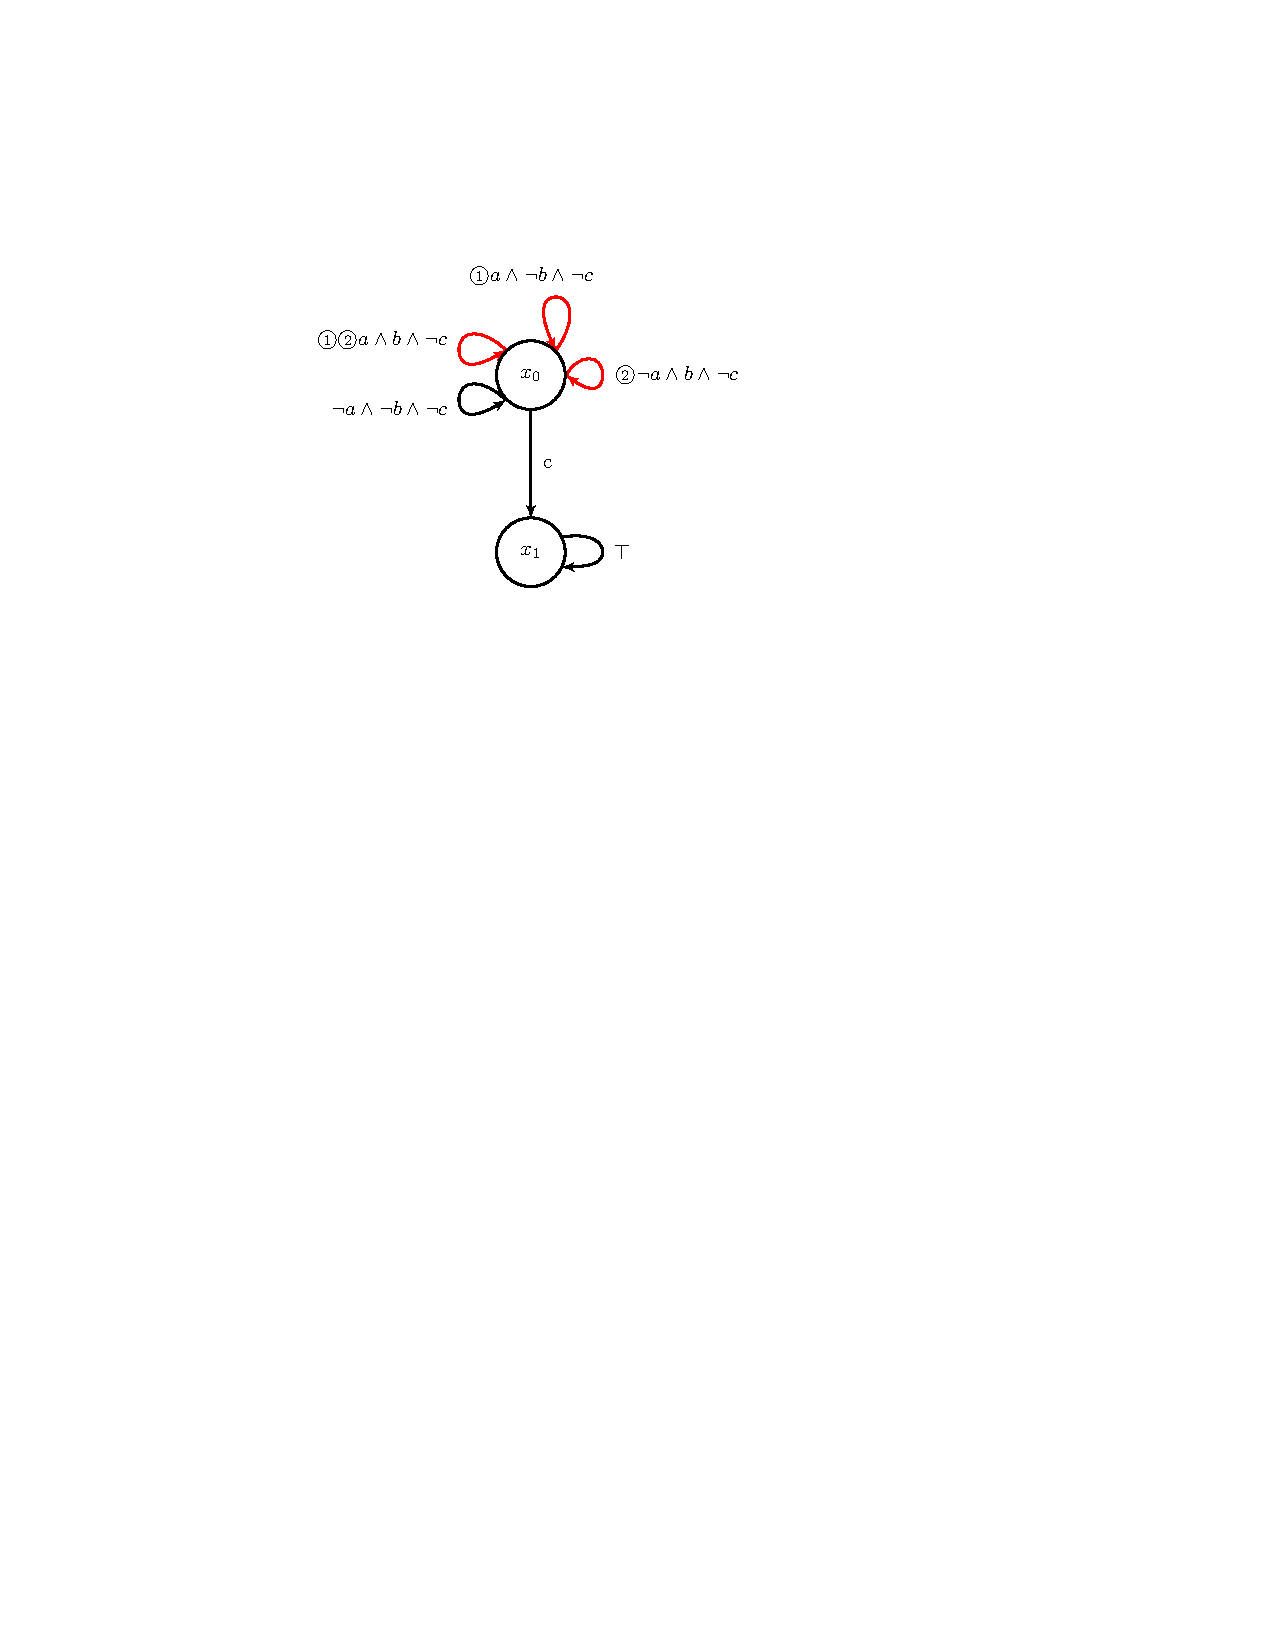
\includegraphics[bb=140 498 368 682,width=5cm]{automaton1.pdf}
   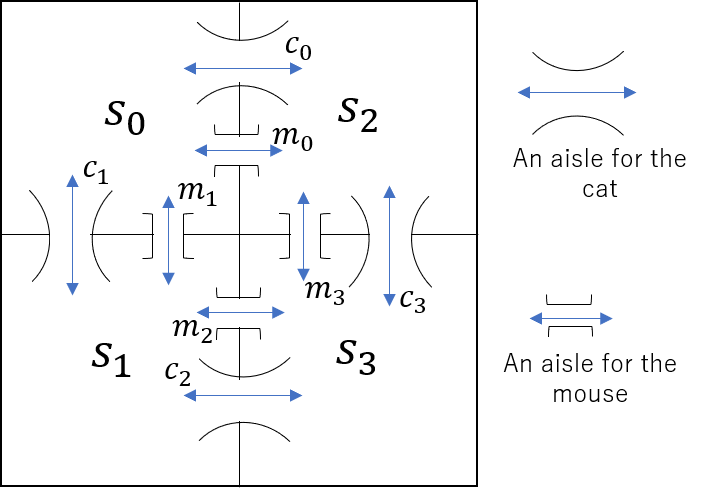
\includegraphics[width = 7cm]{cat_mouse.png}
   \caption{The maze of the cat and the mouse. the initial state of the cat and the mouse is $s_0$ and $s_2$, respectively. the food for them is in the room 1 ($s_1$).}
   \label{cat_mouse}
\end{figure}

\begin{figure}[htbp]
   \centering
   \vspace{2mm}
%   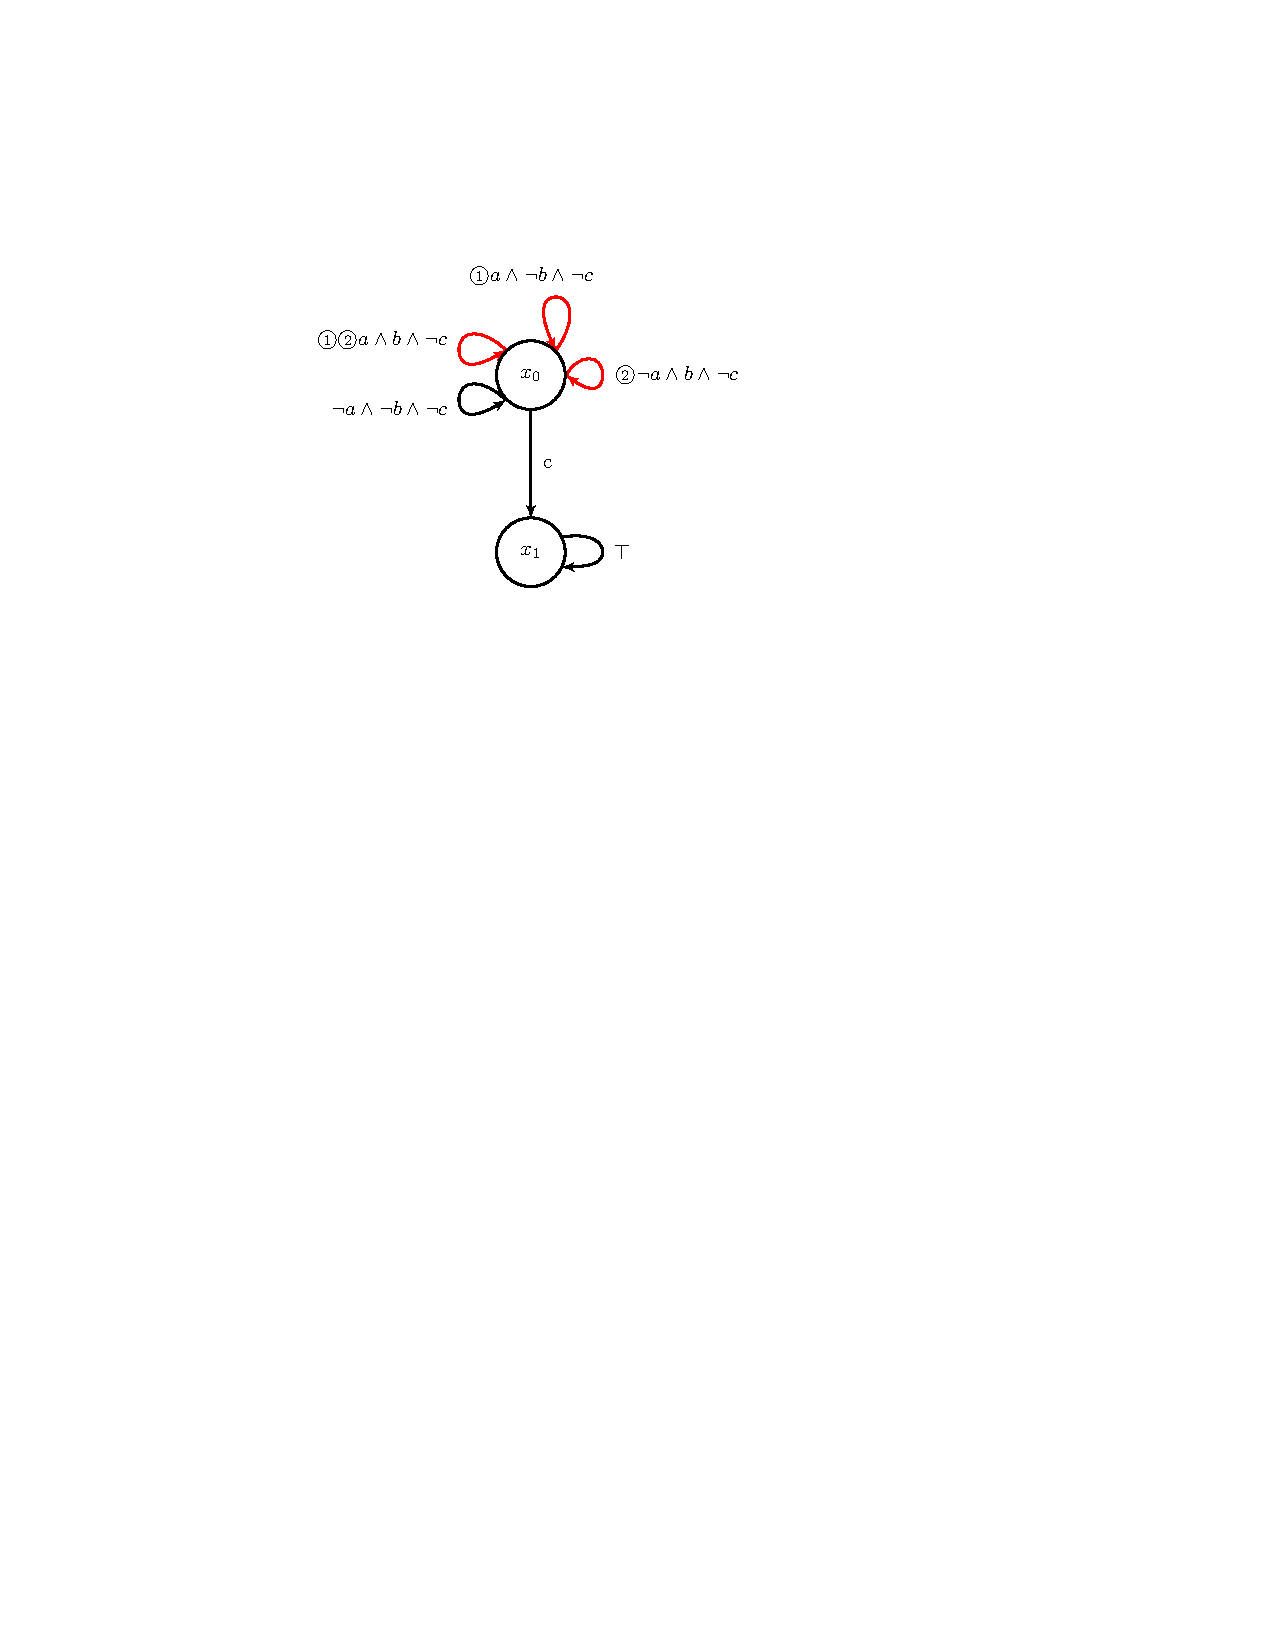
\includegraphics[bb=140 498 368 682,width=5cm]{automaton1.pdf}
   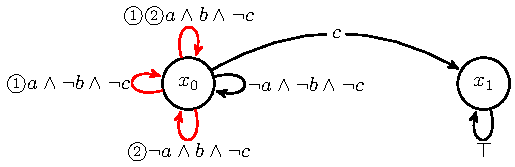
\includegraphics[bb=0 0 247 80,scale=0.85]{ldgba_original.pdf}
   \caption{The tLDBA recognizing the LTL formula $\text{{\bf GF}}a \wedge \text{{\bf GF}}b \wedge \text{{\bf G}}\neg c$, where the initial state is $x_0$. Red arcs are accepting transitions that are numbered in accordance with the accepting sets they belong to, e.g., \textcircled{\scriptsize 1}$a \land \neg b \land \neg c$ means the transition labeled by it belongs to the accepting set $F_1$.}
   \label{tldba}
\end{figure}

\begin{figure}[htbp]
   \centering
   \vspace{2mm}
%   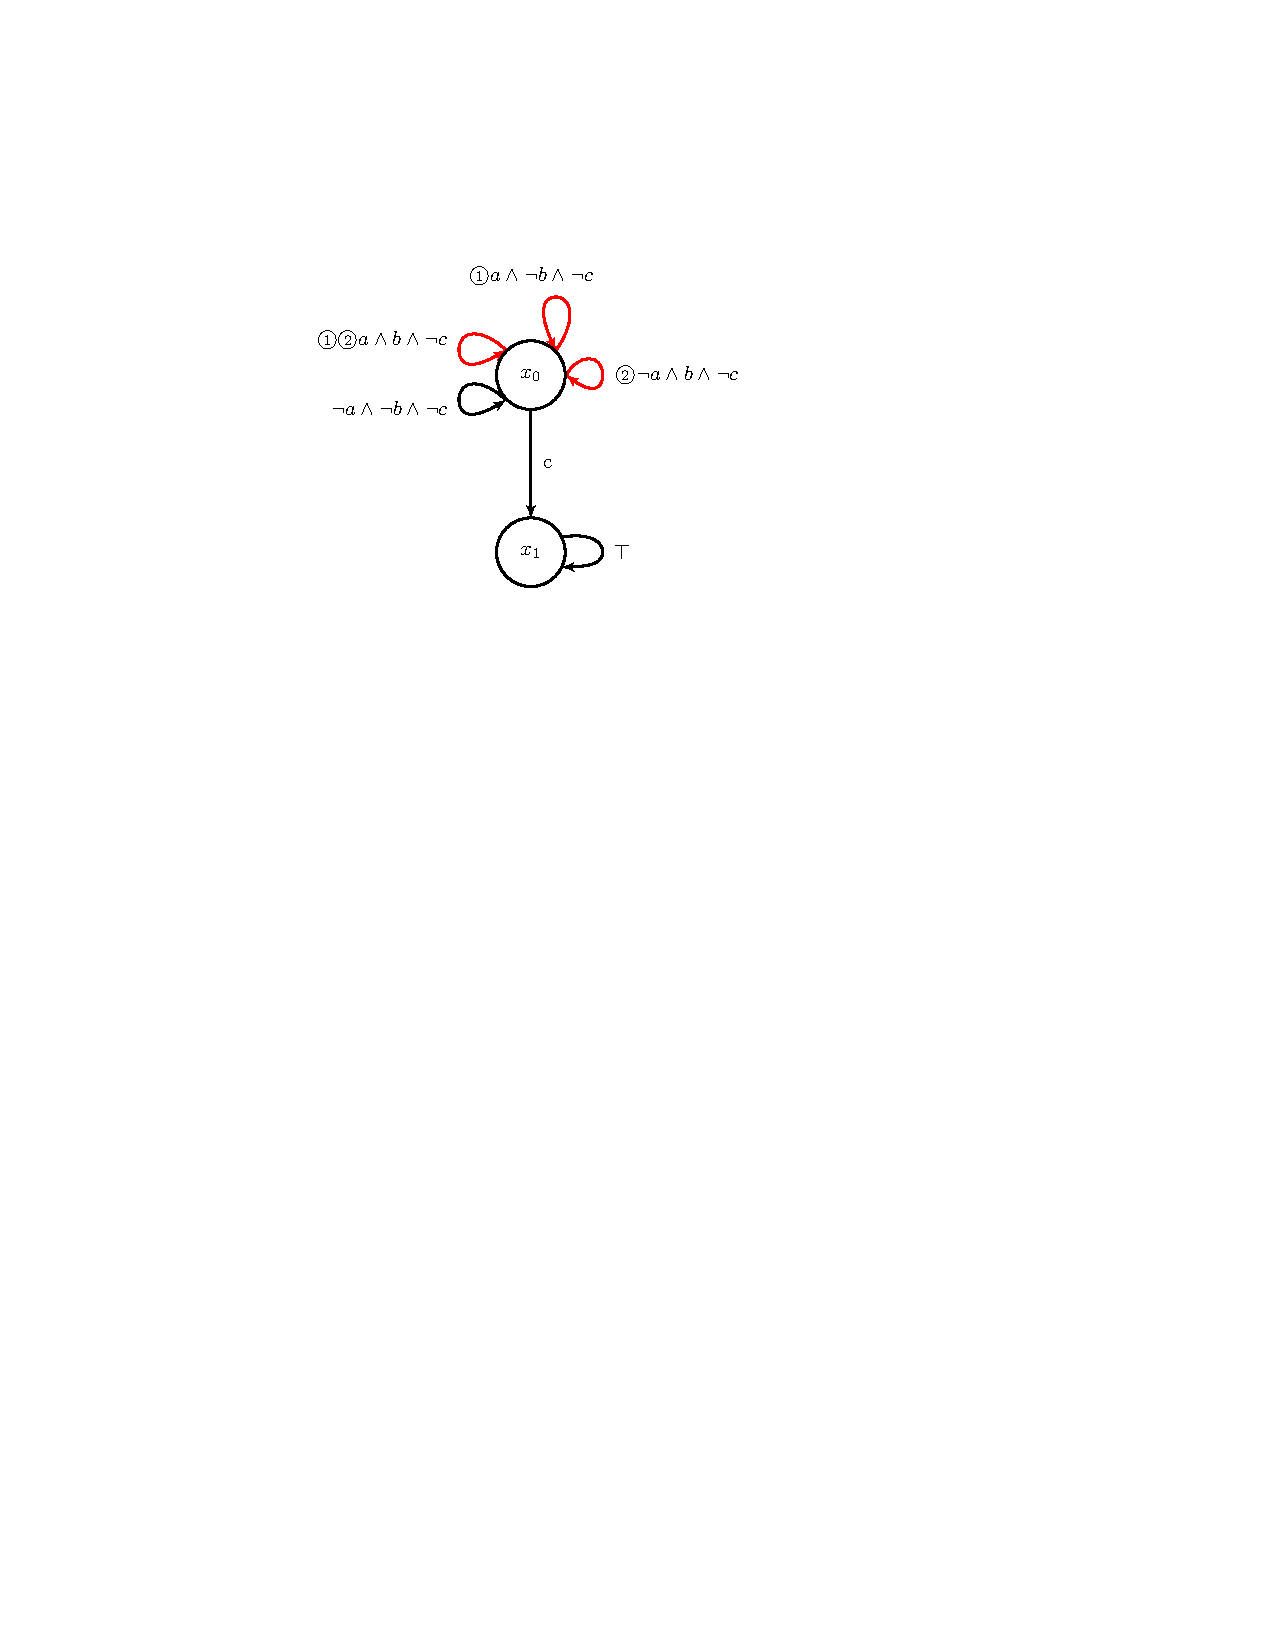
\includegraphics[bb=140 498 368 682,width=5cm]{automaton1.pdf}
   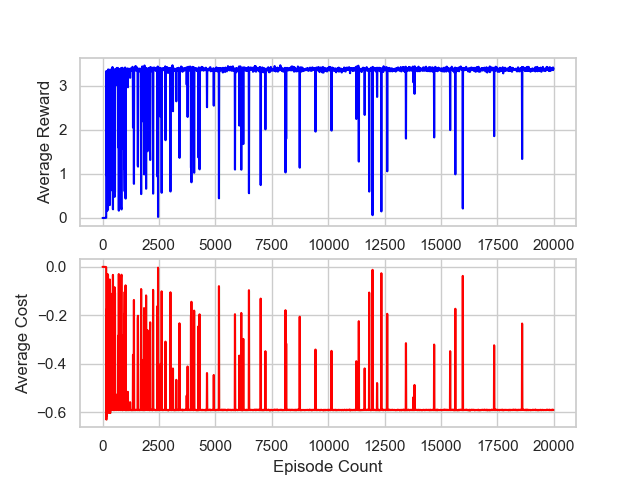
\includegraphics[width = 8cm]{epi20000_step20000_gamma099_ses1_re10_cost01_01_su2.png}
   \caption{The result of the learning when using Algorithm \ref{alg1}.}
   \label{result1}
\end{figure}

\begin{figure}[htbp]
   \centering
   \vspace{2mm}
%   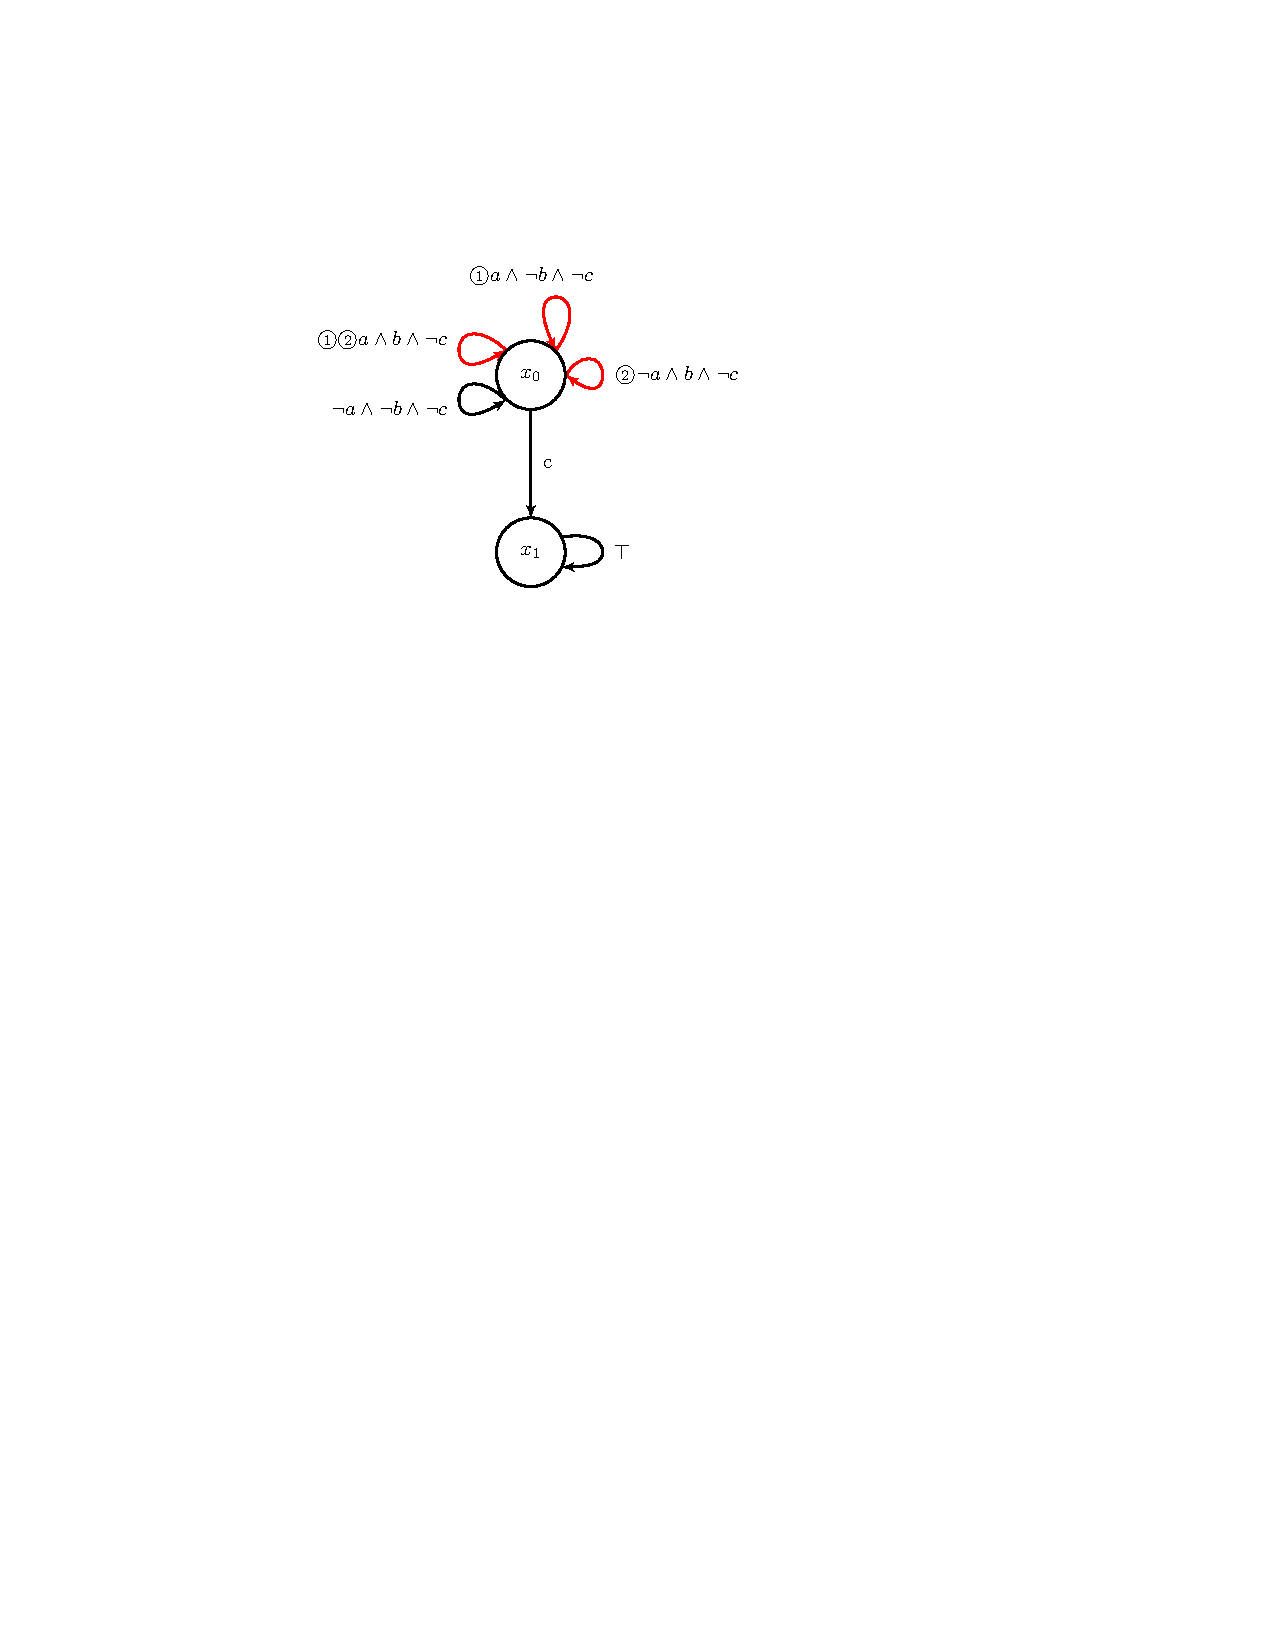
\includegraphics[bb=140 498 368 682,width=5cm]{automaton1.pdf}
   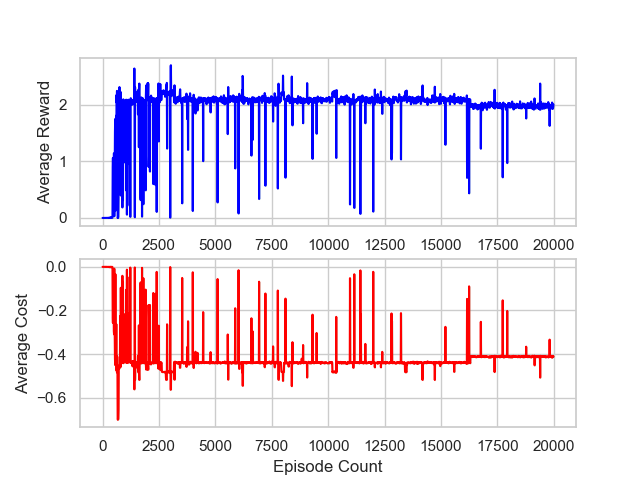
\includegraphics[width = 8cm]{epi20000_step20000_gamma099_ses1_re10_cost01_01_Q-T_su2.png}
   \caption{The result of the learning when using Algorithm \ref{alg2}.}
   \label{result2}
\end{figure}

\begin{comment}
\begin{align}
   L((s, a, s^{\prime})) =
    \left\{
    \begin{aligned}
      & \{ a \} &  & \text{if }s_c^{\prime} = s_1, \nonumber \\
      & \{ b \} &  & \text{if }s_m^{\prime} = s_1, \nonumber \\
      & \{ c \} &  & \text{if }s_c^{\prime} = s_2, \nonumber \\
      & \{ d \} &  & \text{if }s_m^{\prime} = s_4, \nonumber \\
      & \{ e \} &  & \text{if }s_c^{\prime} = s_m^{\prime}, \nonumber \\
      & \emptyset &  & \text{otherwise},
    \end{aligned}
    \right.
\end{align}
where $s_c^{\prime}$ and $s_m^{\prime}$ is the next room where the cat and mouse is, respectively, i.e., $s^{\prime} = (s_c^{\prime},s_m^{\prime})$.

In the example, we want the supervisor to learn to give control patterns satisfying that the cat and the mouse take the food in room 1 ($s_1$) back to each room ($s_2$ and $s_4$) avoiding they come across. This is formally specified by the following LTL formula.
\begin{align*}
  \varphi = \text{{\bf GF}}a \wedge \text{{\bf GF}}b \wedge \text{{\bf GF}}c \wedge \text{{\bf GF}}d \wedge \text{{\bf G}}\neg e.
\end{align*}
The tLDBA $B_{\varphi} = (X, x_{init},\Sigma,\delta,\mathcal{F})$ corresponding to $\varphi$ is shown in Fig.\ \ref{tLDBA}.
\end{comment}


\end{document}
